\documentclass[twocolumn,linenumbers]{aastex631}
\usepackage{amsmath}

% H lines
\newcommand{\halpha}{H$\alpha$}
\newcommand{\hbeta}{H$\beta$}
\newcommand{\hgamma}{H$\gamma$}
\newcommand{\hdelta}{H$\delta$}

%Parameters
\newcommand{\av}{A$_{\text{V}}$}
\newcommand{\mdot}{$\dot{\text{M}}$}
\newcommand{\Mdot}{{\dot{{M}}}}

\newcommand{\msun}{ M_{\sun}}
\newcommand{\rsun}{ R_{\sun}}
\newcommand{\lsun}{ L_{\sun}}
\newcommand{\msunyr}{M_{\sun} \, \rm{ yr^{-1}}}
\newcommand{\kms}{ \, km \, s^{-1}}
\newcommand{\teff}{T$_{\rm eff}$}

% Magnetospheric accretion parameters
\newcommand{\ri}{R$_{\rm i}$}
\newcommand{\rw}{W$_{\rm r}$}
\newcommand{\Dr}{$\Delta \rm r$}
\newcommand{\tmax}{T$_{\rm max}$}
\newcommand{\cosi}{$\cos(i)$}
\newcommand{\lhalpha}{L$_{\rm H\alpha}$}

%\newcommand{\nuria [1]{{\color{green} #1}}}

\received{---- --, ----}
\revised{---- --, ----}
\accepted{---- --, ----}
\submitjournal{}

\begin{document}

\title{Understanding Balmer Decrements in T-Tauri stars in terms of Multi-column Magnetospheric Accretion: Orion OB1b Association}

\correspondingauthor{Naiara Patiño}
\email{naiarap@umich.edu}

\author[0009-0009-7455-6777]{Naiara Patiño}
\affiliation{Institute for Astrophysical Research, Department of Astronomy, Boston University, 725 Commonwealth Avenue, Boston, MA 02215, USA}

\author[0000-0002-3950-5386]{Nuria Calvet}
\affiliation{Department of Astronomy, University of Michigan, 1085 South University Avenue, Ann Arbor, MI 48109, USA}

\author[0000-0000-0000-0000]{Gladis Magris}
\affiliation{Centro de Investigaciones de Astronomía (CIDA), Mérida, 5101, Venezuela.}

\author[0000-0001-8022-4378]{Marbely Micolta}
\affiliation{Department of Astronomy, University of Michigan, 1085 South University Avenue, Ann Arbor, MI 48109, USA}

\author[0000-0003-4507-1710]{Thanawuth Thanathibodee}
\affiliation{Institute for Astrophysical Research, Department of Astronomy,
Boston University, 725 Commonwealth Avenue, Boston, MA 02215, USA}

\author[0000-0002-5231-7240]{Thomas K. Waters}
\affiliation{Department of Astronomy, University of Michigan, 1085 South University Avenue, Ann Arbor, MI 48109, USA}


\shorttitle{algo}
\shortauthors{Patiño et al.}

\begin{abstract}

 :(
    
\end{abstract}

\keywords{stars and stuff}

\section{Introduction}

T-Tauri stars are low-mass stars with spectral types M-K (cite). They are formed from the collapse of gas clouds into a protostar. Studying the physical processes happening in these stars is crucial to understand the evolution of protoplanetary disks and planets. One of the most important processes happening in T-Tauri stars is mass accretion. The current paradigm for this is magnetospheric accretion as described by \citep{hartmann2016}. In this paradigm mass is accreted from the disk in columns following the magnetic field lines of the host star. There is evidence supporting this model such as broad emission lines \citep{muzerolle2001} and UV excess due to the shock of the accreted material unto the star \citep{calvet_gullbring1998}. The study of the emission lines is important for identifying and measuring mass accretion rates (Hartmann 1994, Muzerolle 1998a, 1998b, 2001, white basri 2003).

When modeling emission from accretion columns it is necessary to fit optical and NUV emission because fitting only blue wavelengths have been shown to underestimate mass accretion rates (Fischer 2011). Multicolumn accretion shock models can explain NUV and optical emission simultaneously (Ingleby 2013).

In this work we will study T-Tauri stars from the Orion OB1b region, previously studied by Manara (2021a). This population was chosen because it is in a intermediate level of disk evolution and it is one of the better studied star-forming region. 

This paper is structured as follows. In \ref{Sample and observations} we discuss the sample of T-Tauri stars and characteristics of the population, as well as the details and origin of the observational data used. In \ref{Models} we expand on the details of the magnetospheric accretion model used to fit the observations. In \ref{DataAnalysis} we describe the methodology used to analyse these data, corrections, and statistical methods to obtain our results. Lastly, we discuss our results and their implications in \ref{Discussion}



\section{Observations} \label{Sample and observations}

\subsection{Targets}
The objects studied in this paper are the TTS of the Orion OB1b association observed in the PENELLOPE Large Program by \citep{manara2021}. This part of the ULLYSES program (Roman-Duval 2020). The original sample consisted of 10 CTTS stars. CVSO 104 and CVSO 165 have visual companions \citep{manara2021a}. The primary component of the latter was found to be a spectroscopic binary but could not be resolved (check). On the other hand, CVSO 165 primary component is also a binary stellar system in which both were resolved and had signs of active accretion (check), so they were included in this study. The OB1 association is one of the closest and most populous OB associations, and their subassociations have ages that go from $1Myr-10Myr$ to \citep{blaauw1994}.  We will use the stellar parameters reported by Manara 2021, which were determined using the methods described in \citep{manara2013a}. This consists on fitting the object's dereddened spectra with a hydrogen slab model and a photospheric emission template, in order to reproduce excess emission. Distances were determined using GAIA EDR3 (gaia colab 2016, 2021). All of these parameters are reported in Table -. 

\subsection{X-Shooter spectra}

The observations were made by the PENELLOPE program with the X-Shooter spectrograph in the Very Large Telescope (VLT, Vernet 2021). This instrument has medium-resolution broad-wavelength coverage and is flux-calibrated. Its coverage goes from approx $300-2500nm$  which is important because something. 

\begin{table}[]
\caption{Stellar parameters of the WTTS sample}
\centering

\begin{tabular}{ccccccc}
\hline
Nombre          & SpT  & $d$ {[}pc{]} & M {[}$M_*${]} & $T_{eff}$ {[}K{]} & Log $L/L_{\odot}$ & Ref  \\ \hline
TWA9A          & K5   & 68           & 0.81          & 4350              & -0.61             & M13  \\
RXJ1540.7-3756 & K6   & 150          & --            & 4205              & -0.41             & M17a \\
SO879          & K7   & 360          & 1.07          & 4060              & -0.29             & M13  \\
TWA25          & M0   & 54           & 0.84          & 3850              & -0.61             & M13  \\
TWA14          & M0.5 & 96           & 0.73          & 3780              & -0.83             & M13  \\
TWA13B         & M1   & 59           & 0.68          & 3705              & -0.70             & M13  \\
TWA2A          & M2   & 47           & 0.55          & 3560              & -0.48             & M13  \\
TWA9B          & M3   & 68           & 0.37          & 3415              & -1.17             & M13  \\
TWA15A         & M3.5 & 111          & 0.30          & 3340              & -0.95             & M13  \\
Sz94           & M4   & 200          & 0.28          & 3270              & -0.76             & M13  \\
SO797          & M4.5 & 360          & 0.19          & 3200              & -1.26             & M13  \\
Par-Lup3-2     & M5   & 200          & 0.18          & 3125              & -0.75             & M13  \\
SO999          & M5.5 & 360          & 0.13          & 3060              & -1.28             & M13  \\ \hline
\end{tabular}
  % % }
  %   \begin{tablenotes}
  %           \small
  %           % \item \textbf{Nota.} Las distancias reportadas por \citet{Manara2013} y \citet{Manara2017a} se obtuvieron para los objetos de TW Hya por \citet{Weinberger2013, Torres2008, Mamajek2005}, para $\sigma$ Ori de  \citet{Brown1994} y para Lupus III de \citet{Comeron2008}.
  %   \end{tablenotes}

    \label{SP WTTS}
\end{table}
 
\section{Model} \label{Models}

Magnetospheric accretion model \citep{muzerolle2001}. Description of parameter space.

\begin{table}[]
\centering
\caption{Model stellar parameters}
\begin{tabular}{ccccc}
\hline
SpT & Teff {[}K{]} & L {[}$L_{\odot}${]} & R {[}$R_{\odot}${]} & M {[}$M_{\odot}${]} \\ \hline
K5  & 4350         & 0.745               & 1.519               & 0.872               \\
K7  & 4060         & 0.515               & 1.451               & 0.726               \\
M1  & 3705         & 0.345               & 1.426               & 0.614               \\
M3  & 3415         & 0.215               & 1.327               & 0.465               \\
M5  & 3125         & 0.117               & 1.171               & 0.306               \\ \hline
\end{tabular}
\label{table:parametros_modelos}
\end{table}

Profile of emission lines were calculated from the accretion model proposed by \citet{muzerolle2001}. This uses the extended Sobolev method to simplify calculations. In this case, the radiation field is described by a local radiation and a non-local term. More details of this model are described in the original paper. We used a model grid of 5 stars with stellar parameters in \ref{table:parametros_modelos}. Each of the models of the grid are defined by a combination of accretion parameters: accretion rate ($\dot{M}$), maximum temperature ($T_{max}$), truncation radius ($R_i$), width of the accretion flows at the mid plane ($\Delta R$) and the inclination of the disk ($i$). The geometry of the accretion flows considered in this work is described in \ref{fig:model_geometry}.  The ranges of the parameter space used for this work are described here. The conditions for the accretion rate and maximum temperature come from \citet{muzerolle2001}.  It is important to note that this model assumes dipolar geometry and axisymmetry of the magnetic field. 

\begin{itemize}
    \item $-10 \leq \msunyr log(\Mdot) \leq -7\msunyr$ in steps of $log(0.25) \msunyr$
    \item $6500 K \leq$ \tmax $\leq 14000 K$ in steps of $500 K$.
    \item $2 R_* \leq$ \ri $\leq 6 R_*$ in steps of $0.5 R_*$
    \item \Dr $= 0.5 R_*$, $1 R_*$, $2 R_*$
\end{itemize}

\begin{figure}
    \centering
    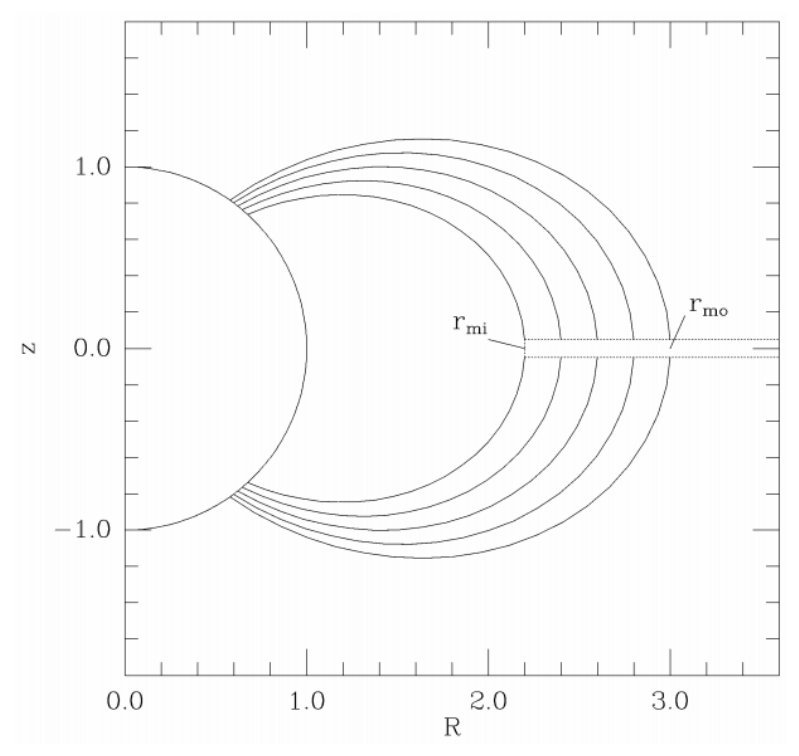
\includegraphics[width=0.75\linewidth]{figures/geometry.png}
    \caption{Model geometry}
    \label{fig:model_geometry}
\end{figure}

\section{Multicolumn accretion}

Several studies indicate that stellar magnetic fields are far from dipolar and axisymmetric (cite). Simulations for more complex magnetic field geometry exist (see \citet{romanova2003}) but an analytical model doesn't exist (check atom 2023). Using the model grid as is has been insufficient to explain the observed Balmer fluxes in previous works (cite) as it underpredicts \hgamma emission. We try to replicate these fluxes and account more accurately for the complexity of the accretion flows by assuming two accretion columns of different densities. Each would have different emission areas, fractions of the total emission area of the flows. There is observational evidence of these density gradients as shown in \citet{}

 The concept of multiple column accretion has been applied before to the model of accretion shock by \citet{pittman2022} and others. They were able to explain observations of shock emission using columns of different energy densities. 

\begin{figure}
    \centering
    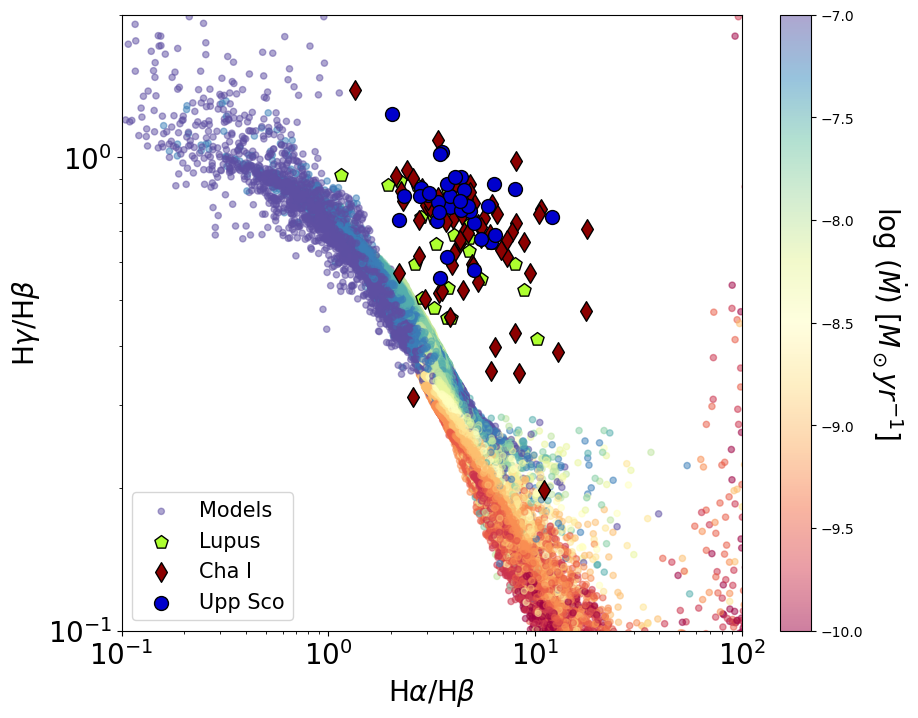
\includegraphics[width=0.8\linewidth]{figures/BalmerDecrements.png}
    \caption{Balmer decrements}
    \label{fig:balmer_decrement}
\end{figure}

The observed Balmer decrements of different regions do not correspond to the Balmer decrements obtained from the model grid, as can be seen in figure tal. Given that, we tested whether those could be reproduced by combining the lines fluxes of two different models from the grid weighed by a factor $f_i$ for each model. These factors represent the fraction of the emitting area covered by a given column or accretion flow. We fixed the factor for one of the models $f_1=10^{-3}$ and tried different values of factors for the other model, $f_2 = 10^{-1},10^{-2},10^{-4}$ .  Those factors were chosen based on the \textit{filling factors} of the accretion shock model. Though those factors are not equivalent, they represent a similar concepts. In the case of filling factors in the accretion shock model, they are interpreted as the percentage of the star surface that is covered by the emission from the shock.

As a test of this idea, we defined a region in the Balmer decrement diagram on which most of the observation fell. Then, we tried different combinations of models and checked if, when weighed by $f_i$, the decrement of the combined models could reproduce the observed ones, meaning that it would fall on the defined region on the Balmer diagram. When looking at the parameter distribution of these two models separately, we can observe certain tendencies. We will refer to each of these models as 'columns' to make the discussion easier. The column covering the smaller area tends to have higher accretion rates, while the larger one tends to have lower accretion rates. That corresponds to a higher density and smaller column and a lower density and larger column.

\section{Data analysis}

\subsection{Line fluxes}

Extinction correction, heliocentric velocity, flux calculations, errors

Fluxes of emission lines were calculated integrating the spectra after extinction and heliocentric velocity correction and after subtracting the continua determined using this package. The errors were calculated following the method outlined by \citet{alcala2014}. This method consists of determining two more continua, one higher and lower than the middle one. In this case, we used 10\% difference between the central and the other continua. The total line flux was calculated from the average of the flux calculations using the three different continua and the error was the standard deviation $\sigma$. The emission lines analyzed in this work were \halpha, \hbeta and \hgamma.


\subsection{MCMC}

why bayesian statistics and why MCMC. Characteristics of the MCMC used. 

We used MCMC with 10000 steps and 50 walkers from the package \textit{emcee}

\subsection{Profile fitting}

After sampling with the MCMC, we took the final samples and took the ones with a likelihood over the \% . The profiles of those models was compared to the observations and best fits were found minimizing $\chi^2$ of the three Balmer lines simultaneously.

\section{Results}

Previous works using the same model grid, found a systematic underestimation of the flux of \hgamma. One of the goals of this work was to solve this issue using a combination of models. This tries to represent the complexity of real stellar magnetic field by combining high-density and low-density accretion flows covering different fractions of the total area covered on the stellar surface.

Sampling using the MCMC methods we were able to find model combinations that could reproduce more accurately observed fluxes of the three Balmer lines studied, solving the issue of \hgamma.

It appears that \hgamma is forming mainly in the higher density columns, which almost make no contirbution to the total flux of \halpha. 

Can we see trends in the parameters of the best fits?

\section{Discussion} \label{Discussion}

Magnetic fields geometry is complex and a one column accretion model cannot explain the observations. Using two columns we can explain the observed line fluxes. This is a rough approximation to the reality of complex magnetic fields.

Density structure in \citet{zhaohuan2024}, \citet{espaillat2021}

Variability of accretion. "These stars show complicated spectral variability patterns which may be connected with the structure of the magnetospheric flows" \citep{romanova2003}

Magnetospheric flows absorb light from photosphere and chromosphere? \citep{atom2023}

\section*{Acknowledgements}

Thanks Katya

\software{Astropy, ...}

\bibliography{references.bib}{}
\bibliographystyle{aasjournal}

\end{document}
